\chapter{Entwurfsmuster}

\section{Entwurfsmuster: Fabrik}

\section{Entwurfsmuster: Kompositum}

Die nachfolgende Abbildung zeigt das UML-Diagramm der Klassen
\textit{Buffer} und \textit{CompositeBuffer}, wobei letztere von
ersterer erbt. Beide Klassen finden Verwendung in der Spielanzeige
auf der Konsole. Dabei werden statische \textit{Sprites} mithilfe
der Klasse \textit{Buffer} beschrieben, komplexere Anzeigen, bei denen
dynamische Änderungen auftreten können mithilfe der Klasse
\textit{CompositeBuffer}.

Es handelt sich hierbei um das Entwurfsmuster \textbf{Kompositum}. 
Objekte der beiden Klassen lassen sich gemeinsam zu einer Baum-Struktur
zusammensetzen. Beide Typen sind gleichwertige Komponenten. Die
\textit{Buffer} sind dabei Blätter bzw. einfache Elemente, wohingegen
\textit{CompositeBuffer} wie Container funktionieren und die Kinder
verwalten. 

In der Gesamtheit verhalten sie sich wie eine Einheit. Sie teilen sich
alle Funktionen der zugrundeliegenden Klasse \textit{Buffer}. So etwa
die Funktion \textit{toString()}, welche den Buffer-Inhalt in einen
String für die Konsole überführt oder die Funktion \textit{render()},
welche rekursiv den Baum vom Wurzel-Element ausgehend traversiert und
entsprechende Updates veranlasst.

In der Abbildung ist zu sehen, dass die Klasse
\textit{CompositeBuffer} genutzt wird, um Anzeigen (\textit{Views})
zu erstellen. Die bedeutenste Klasse ist dabei
\textit{TerminalInterface}, da sie die Hauptanzeige modelliert.
Die Klasse \textit{CompositeBuffer} bietet jedoch, im Gegensatz zum
\textit{Buffer}, zur Einfachheit und Effizienz die Möglichkeit
zwischen fixierten \textit{fixed()} und dynamischen \textit{dynamic()}
Elementen zu unterscheiden.

\vspace{0.5cm}
\begin{figure}[H]
    \centering
    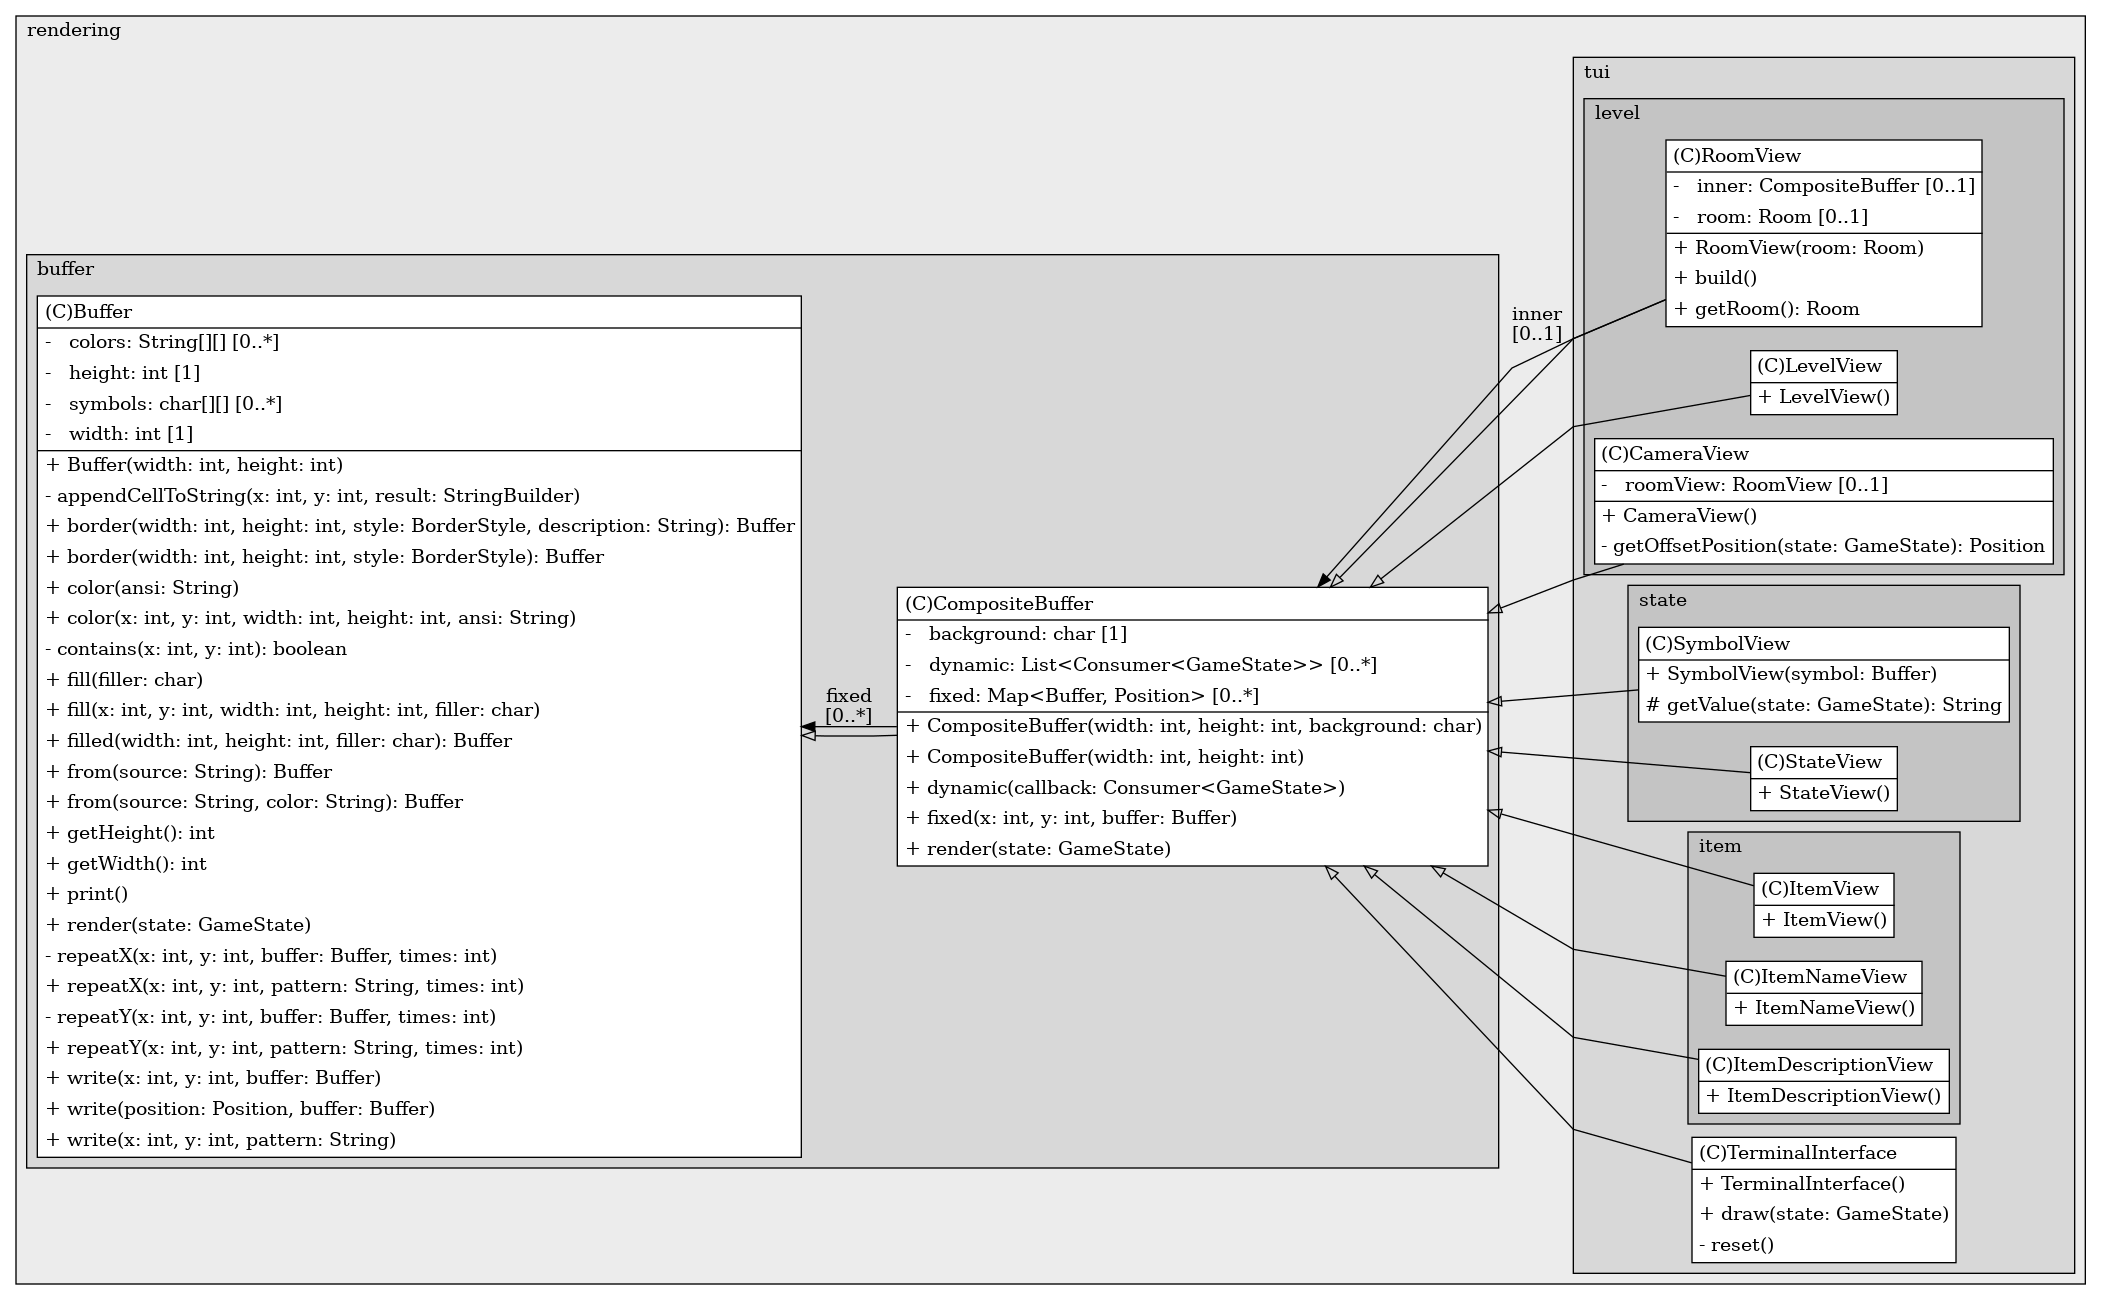
\includegraphics[width=1\linewidth]{Bilder/Visualisierung/CompositeBuffer_structure.png}
    \caption{KeyInputHandlerFake}
\end{figure}